\chapter{气体动理论}
\section{选择题}
\exercise B

\solve 微观上,气体温度表示气体分子的运动速度,对于单个或少数分子,温度的概念失去了意义。宏观上,气体的温度表示气体分子的平均冷热程度。

\exercise B

\solve
\begin{gather*} 
{v_p=\sqrt{\frac{2kT}{u}}}\\
{u\left(\ce{O2}\right)}>u\left(\ce{H2}\right)\\
{v_p\left(\ce{O2}\right)<v_p\left(\ce{H2}\right) } \\
\frac{v_p\left(\ce{O2}\right)}{v_p\left(\ce{H2}\right)}=\sqrt{\frac{2kT}{32}}{\displaystyle\Huge/} \sqrt{\frac{2kT}{2}}=\frac{1}{4}%需要长斜杠分数线
\end{gather*}
$k$为常量,$T$相同。

\exercise C

\solve 自由度为$i$的分子的平均动能为$ikT/2$。

\exercise A

\solve

$$
\begin{aligned} 
\sqrt {\overline{v^{2}}} &=\sqrt{\frac{3kT}{u}} \\
u\left(\ce{H2}\right)& > u\left(\ce{H2}\right) \\
\sqrt {\bar{v^2}\left(\ce{O2}\right)}& = \sqrt {\bar{v^2}\left(\ce{H2}\right) }\\
T\left(\ce{O2}\right)&>T\left(\ce{H2}\right) 
\end{aligned}
$$

\exercise B

\solve 等温过程系统内能不变。

\exercise A

\solve

\begin{gather*}
\varepsilon_{\ce{He}}=\varepsilon_{\ce{N2}}\\
n_{\ce{He}}=n_{\ce{N2}}\quad n=\frac{N}{V}\\
\bar{\varepsilon}=\frac{3}{2}kT\\
T_{\ce{He}}=T_{\ce{N2}}\\
p=\frac{2}{3}n\bar{\varepsilon}\\
p_{\ce{He}}=p_{\ce{N2}}
\end{gather*}

\exercise A

\solve

$$
\begin{aligned} 
p V & = \nu R T \\ p V & = \frac { m } { M } R T \\
p V & = \rho R T \\
\rho & = \frac { p M } { R T }
\end{aligned}
$$

由于水滴静止,则
$$
p_{\ce{H2}} =p_{\ce{O2}}
$$

又因为T相同,则

$$
\frac { p_{\ce{H2}} } { p _{\ce{O2}} } = \frac { \frac { p M _ {\ce{H2}} } { R T } } { \frac { p M_{\ce{O2}}}{ R T}}=\frac{1}{16}
$$

\exercise D

\solve

$$
\begin{aligned}
 \bar { z } & = \sqrt { 2 } \pi d ^ { 2 } \bar { v } n \\ \lambda & = \frac { 1 } { \sqrt { 2 } \pi d ^ { 2 } n } 
\end{aligned}
$$

$$
\because n = \frac { p } { k T }
$$不变,$ \bar { v }$不变

$$
\bar { z } = \sqrt { 2 } \pi d ^ { 2 } \bar { v } \frac { p } { k T },p
$$变为原来的两倍

$$
\begin{array} { l } 
{ \therefore z ^ { \prime } = 2 \bar { z } } \\ 
{ \because \bar { v } = \bar { \lambda } \bar { z } } \\
 { \therefore \lambda ^ { \prime } = 2 \bar { \lambda } }
\end{array}
$$

\exercise C

\solve

$$
\begin{array} { l } 
{ 2\ce{H2O} = 2\ce{H2}+\ce{O2}}\\
{ E = v\frac{i}{2}RT} 
\end{array}
$$

对于刚性分子,双原子分子气体的i=5,多原子分子气体的i=6

$$
\begin{array} { l }
 E _ { 0 } = 2 \cdot \frac { 6 } { 2 } R T \\ E _ { 0 } ^ { \prime } = 2 \cdot \frac { 5 } { 2 } R T + \frac { 5 } { 2 } R T = \frac { 15 } { 2 } R T \\ \therefore \frac { 15 } { 2 } R T \div 6 R T = 125 \% 
\end{array}
$$

\exercise B

\solve

$$
\begin{aligned} 
\sqrt { \bar { v } ^ { 2 } } & = \sqrt { \frac { 3 k T } { u } } \\ T _ { 2 } & = \frac { 3 } { 2 } T _ { 1 } \\ T _ { 2 } = \left( \frac { 3 } { 2 } \right) ^ { 2 } T _ { 1 } & = 280 \times \frac { 9 } { 4 } = 630 
\end{aligned}
$$
\section{填空题}
\exercise 
$\int _ { v _ { 2 } } ^ { v _ { 2 } } f ( v ) N\di{v}$
\qquad
$\frac { \int _ { v _ { 1 } } ^ { v _ { 2 } } v f ( v )\di{v}} { \int _ { v _ { 1 } } ^ { v _ { 2 } } f ( v )\di{v}}$
\qquad
$N \cdot \frac { 1 } { 2 } m \int _{v_1}^{v_ 2} v^2f( v )\di{v}$

\solve
(1)

$$
\begin{aligned}
\frac { d N } { N } & = f ( v ) d v \\ d N & = N f ( v )\di{v}\\ N ^ { \prime } = & \int _ { v_1 } ^ { v _ { 2 } } N f ( v )\di{v}
\end{aligned}
$$

(2)
$$
\begin{aligned}
v_1 \sim v_2 \mbox{的平均速度}&=\frac{\mbox{这个区间里每个分子速度之和}}{\mbox{这个区间里分子总数}}\\
&=\frac { \int _ { v _ { 1 } } ^ { v _ { 2 } } v\di{N}} { \int _ { v _ { 1 } } ^ { v _ { 2 } }\di{N}} = \frac { N \int _ { v _ { 1 } } ^ { v _ { 2 } } v f ( v )\di{v}} { N \int _ { v _ { 1 } } ^ { v _ { 2 } } f ( v )\di{v}} \\
&=frac { \int _ { v _ {1 } } ^ { v _ { 2 } } v f ( v )\di{v}} { \int _ { v _ { 1 } } ^ { v _ { 2 } } f ( v )\di{v}}
\end{aligned}
$$

(3)
$$
\begin{aligned}
\mbox{总平动动能之和=每个分子平动动能之和}&= \int _ { v _ { 1 } } ^ { v _ { 2 } } \frac { 1 } { 2 } m v ^ { 2 }\di{N}\\
&=\frac{1}{2}m N \int _ { v _ { 1 } } ^ { v _ { 2 } } v ^ { 2 } f ( v )\di{v}
\end{aligned}
$$


\exercise $\frac { N _ { A } } { N _ { A } + N _ { B } } f _ { A } ( v ) + \frac { N _ { B } } { N _ { A } + N _ { B } } f _ { B } ( v )$

\solve $\frac{N_A}{N_A+N_B}$指的是A在混合气体里占比,B同理。由概率论知识可知,对概率密度求加权平均即得结果。



\exercise
$n _ { 0 } e ^ { - \frac { m g z } { k T } } \qquad z = - \frac { k T \ln ^ { \frac { p } { p_0 } } } { m g }$

\solve 由玻尔兹曼分布律:

$$
\begin{aligned}
n & = n _ { 0 } e ^ { - \frac { m g z } { k T } } \\ p & = p _ { 0 } e ^ { - \frac { m g z } { k T } } \\ z & = - \frac { k T \ln ^ { \frac { p } { p _ { 0 } } } } { m g } \end{aligned}
$$

\exercise 升高\qquad 升高

\solve (1)温度应上升。因为高速运动的氧气瓶中的分子是在杂乱无章运动的基础上附加上x方向定向运动速度。氧气瓶静止下来后,气体分子与氧气瓶发生碰撞,高速的x方向定向运动动能通过分子之间的频繁碰撞逐步平均分配到y、z方向的热运动动能上去,所以温度上升。

(2)$pV=\nu RT$,$T$增大,$V,\nu,R$都不变,所以$p$增大。

\exercise $\frac{3kT}{2}$\qquad 温度是大量分子热运动的集体表现,对单个或少数分子来说,温度的概念就失去了意义。

\exercise $7.82 \times 10 ^ { 7 } s ^ { - 1 } \qquad5 \times 10 ^ { - 5 } \mathrm { cm }$

\solve
由$\bar { \lambda } = \frac { k T } { \sqrt { 2 } \pi d^2p }$,$\bar { \lambda } $和$\bar { v } $成反比.

$p _0= 1 \times 10 ^ { 5 }\mathrm{Pa}$

$p _1= 1 \times 10 ^ { 4 }\mathrm{Pa}$

${ \therefore\ \overline{\lambda^{\prime} } = 10 \bar { \lambda } = 5 \times 10 ^ { - 5 }\mathrm{ cm }}$

${ z ^{\prime } = \frac { 1 } { 10 } \bar { z } = 7.82 \times 10 ^ { 7 }\mathrm{s^{-1}}}$

\exercise 1:4:16\qquad 1:2:4

\solve

$$
\begin{array}{*{20}{c}}
 \sqrt { \bar { v } ^ { 2 } } = 1.73 \sqrt { \frac { R T } { M } } \\ \because \sqrt { \bar { v } _ { A } ^ { 2 } } : \sqrt { \bar { v } _ { B } ^ { 2 } }  : \sqrt { \bar { v } _ { C } ^ { 2 } } = 1 : 2 : 4 \\ \therefore T _ { A } : T _ { B } : T _ { C } = 1 : 2 ^ { 2 } : 4 ^ { 2 } = 1 : 4 : 16 \\ n = \frac { N } { V } = \frac { \nu N _ { A } } { V } \\ \therefore n \propto \frac { \nu } { V }\\ \therefore \frac { \nu _ { 1 } } { V _ { 1 } } : \frac { \nu _ { 2 } } { V _ { 2 } } : \frac { \nu _ { 3 } } { V _ { 3 } }  = n _ { 1 } : n _ { 2 } : n _ { 3 } = 4 : 2 : 1 \\ p V  = \nu R T \\ p = \frac { \nu R T } { V }  = \frac { \nu } { V } \cdot T \cdot R \\ \therefore p  \propto \frac { \nu } { V } T \\ \therefore p _ { 1 } : p _ { 2 } : p _ { 3 } = 4 \times 1 : 2 \times 4 : 1 \times 16 = 1 : 2 : 4  
\end{array}
$$

\exercise 6

\solve (1)刚性多原子分子(甲烷)共有6个自由度。

(2)由于分子热运动的无规则性,任何一种运动都不比其他运动占有特别的优越性,所以机会相等,所以分子绕其质心转动对$i$的贡献为3.

\exercise $\geqslant 0 $\qquad 不变 \qquad 增

\solve
(1)孤立系统的熵永远也不会减少。

(2)可逆过程熵不变。

(3)由于ΔS$\geqslant 0$,不可逆过程熵增。


\exercise 0 \qquad 增

\solve(1)气体自由膨胀,对外界不做功(A=0)。绝热过程Q=0,ΔE=-A=0。故内能增量为0。

(2)孤立系统的熵永远也不会减少。


\section{计算题}
\exercise

\solve
(1)
\begin{figure}[!ht]
	\centering
	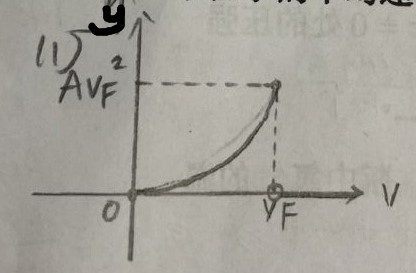
\includegraphics[width=0.35\textwidth]{./pics/Chp12_21.jpg}
\end{figure}

(2)
\begin{align*}
\int _ { 0 } ^ {+\infty}f(v)\di{v}
&=\int _ { 0 } ^ {v_F}Av^2\di{v}\\
&=\left. \dfrac { 1 } { 3 } A v ^ { 3 } \right| _ { 0 } ^ { v _ { F } }\\
&=\dfrac { 1 } { 3 } A v_F^3= 1 \\ 
A&=\dfrac{3}{ v_F^3 }
\end{align*}

(3)
速率分布曲线上与速率分布函数极大值所对应的速率称为最概然速率。

\therefore $v_P=v_F$

(4)
\begin{gather*}
{ \bar { v } = \int _ { 0 } ^ { v _ { F } } v f ( v ) d v } \\
 { \bar { v } = \int _ { 0 } ^ { v _ { F } } v \cdot \frac { 3 } { v _ { F } ^ { 3 } } v ^ { 2 } d v = \left. \frac { 3 } { 4 v _ { F } ^ { 3 } } v ^ { 4 } \right| _ { 0 } ^ { v _ { F } } = \frac { 3 } { 4 } v _ { F } } 
\end{gather*}

(5)
\begin{gather*}
 { \bar { v } = \int _ { 0 } ^ { v _ { F } } v f ( v ) d v } \\
{ \bar { v } = \int _ { 0 } ^ { v _ { F } } v \cdot \frac { 3 } { v _ { F } ^ { 3 } } v ^ { 2 } d v = \left. \frac { 3 } { 4 v _ { F } ^ { 3 } } v ^ { 4 } \right| _ { 0 } ^ { v _ { F } } = \frac { 3 } { 4 } v _ { F } } \\ { \bar { v } ^ { \prime } = \int _ { \frac { v _ { F } } { 2 } } ^ { v _ { F } } \frac { 3 } { v _ { F } ^ { 3 } } v ^ { 3 } d v = \left. \frac { 3 } { 4 v _ { F } ^ { 3 } } v ^ { 4 } \right| _ { \frac { v _ { F } } { 2 } } ^ { v _ { F } } = \frac { 3 } { 4 v _ { F } ^ { 3 } } \left( v _ { F } ^ { 4 } - \frac { 1 } { 16 } v _ { F } ^ { 4 } \right) = \frac { 45 } { 64 } v _ { F } }
\end{gather*}

\exercise

\solve
(1)
\begin{gather*}
{ p = n k T } \\ 
{ n = \frac { p } { k T } = 2.415 \times 10 ^ { 25 } } \\ 
{ n ^ { \prime } = 2.415 \times 10 ^ { 16 } } \\
 { \therefore N = 2.415 \times 10 ^ { 16 } \mbox{个} } 
\end{gather*}

(2)
$$
m _ { 0 } = \frac { M } { N _ { A } } = 5.31 \times 10 ^ { - 23 } g
$$

(3)
\begin{align*}
\rho &= \frac { m } { V } = \frac { N m _ { 0 } } { V }\\
&= \frac { 2.415 \times 10 ^ { 16 } \times 5.31 \times 10 ^ { - 23 } } { 10 ^ { - 9 } } \times 10 ^ { - 3 } \\
&= 1.28236 \times 10 ^ { 27 } \mathrm { kg } / \mathrm {m^3}
\end{align*}

(4)
$$
\bar { v } = \sqrt { \frac { 8 k T } { \pi m _ { 0 } } } = \sqrt { \frac { 8 \times 1.38 \times 10 ^ { - 23 } \times 300 } { \pi \times 5.31 \times 10 ^ { - 23 } \times 10 ^ { - 3 } } } = 446 \mathrm { m } / \mathrm { s }
$$

\exercise

\solve
(1)
\begin{align*}
p &= p _ { 0 } e ^ { - \frac { \mu g h } { k T } } = p _ { 0 } e ^ { - \frac { M g h } { R T } } \\
&= 0.633 p _ { 0 } \\
&= 6.45 \times 10 ^4\mathrm{Pa}
\end{align*}
(2)

每口吸入的空气v不随海拔变化而变化。

相同质量$\Rightarrow v $相同。

$pV=nRT$

忽略气温随高度变化时,T为定值。

$\therefore p_{0}\cdot 17 v =0.633p_0 \cdot x v$

${ x = 26.7 \approx 27}$ 


\exercise

\solve
(1)
$$
\begin{array} { c } { \rho = \frac { m } { V } = \frac { \nu m _ { 0 } } { V } = 11.3 g / c m ^ { 3 } } \\ { p V = \nu R T } \\ { \therefore \frac { \nu } { V } = \frac { p } { R T } = \frac { 1.01 \times 10 ^ { 3 } } { 8.314 \times 300 } = 0.405 } \\ { m _ { 0 } = \rho \frac { V } { \nu } = \frac { 11.3 } { 0.405 } = 27.9012 \approx 28 } \end{array}
$$

则可能是\ce{N2},\ce{CO},\ce{CH2=CH2}

(2)
$$
\sqrt{\bar{v^{2}}}=\sqrt {\frac{3kT}{\mu}}=1.73\sqrt {\frac{RT}{M}}=1.73\times\sqrt{\frac{8.314\times 300}{28\times10^{-3}}}=516.8\mathrm{m}/\mathrm{s}
$$

(3)
\begin{align*}
\bar{\varepsilon_{\mbox{平}}}&=\frac{3}{2}kT\\
&=\frac{3}{2}\times 1.38\times 10^{-23}\times 300\\
&=6.21\times 10^{-21}\\
\bar{\varepsilon_{\mbox{转}}}&=kT\\
&=4.14\times 10^{-21}
\end{align*}

(4)单位体积总平动动能=1个分子平均平动动能*分子数密度

$$E_{\mbox{平总}}=\bar { \varepsilon } _ {\mbox{平}}n=\bar { \varepsilon } _ {\mbox{平}}\frac{p}{kT}=6.21 \times 10 ^ { - 21 } \times \frac { 1.01 \times 10 ^ { 3 } } { 1.38 \times 10 ^ { - 23 } \times 300 } = 1515 J$$

同理,$\bar { \varepsilon } _ {\mbox{转总}}=1010J$

(5)
$$
E = \nu \frac { i } { 2 } R T = 0.3 \times \frac { 5 } { 2 } \times 8.314 \times 300 = 1870.65 J
$$